\chapter{Planificación}

En un sistema multiprogramado, varios procesos residen simultáneamente en memoria principal. Mientras un proceso utiliza el procesador, los demás permanecen esperando la ocurrencia de algún evento o ser seleccionados por el planificador. La planificación (\textit{scheduling}) permite seleccionar qué proceso se ejecutará en cada instante, manteniendo el procesador ocupado y mejorando el rendimiento del sistema.

Existen cuatro tipos de planificación: planificación de largo plazo, de mediano plazo, de corto plazo y de E/S. En este capítulo se estudian únicamente los tres primeros, conocidos en conjunto como \textit{planificación del procesador}.

\section{Tipos de planificación del procesador}

El objetivo de la planificación del procesador es asignar procesos a uno o varios procesadores de manera que se optimicen métricas como el \textit{tiempo de respuesta}, el \textit{rendimiento} (\textit{throughput}) y la \textit{utilización del procesador}. Para ello, la planificación se divide en tres funciones, diferenciadas por la escala temporal en la que actúan:
\begin{itemize}
  \item \textit{Planificación de largo plazo:} decide si un proceso recién creado será admitido al conjunto de procesos activos, controlando el grado de multiprogramación.
  \item \textit{Planificación de mediano plazo:} forma parte del mecanismo de \textit{swapping}. Determina qué procesos permanecen, al menos parcialmente, en memoria principal y cuáles son suspendidos temporalmente.
  \item \textit{Planificación de corto plazo:} selecciona cuál de los procesos en estado \textit{Ready} utilizará el procesador a continuación. Es la función que se ejecuta con mayor frecuencia y la que más influye en el comportamiento inmediato del sistema.
\end{itemize}

\begin{figure}[!ht]
  \centering
  \begin{tikzpicture}[>=Stealth,font=\scriptsize]
    \tikzset{
      state/.style={
        draw,
        thin,
        minimum width=2.1cm,
        align=center,
        minimum height=1.3cm,
        shape=ellipse,
        inner sep=0pt,
        font=\small,
        text=black,
        outer color=white!85!green!85!blue,
        inner color=white,
        outer sep=.1cm
      }
    }
    \node[state] (sready) {Listo\\Suspendido};
    \node[state, right=1.3cm of sready] (ready) {Listo};
    \node[state, below=2cm of ready] (blocked) {Bloqueado};
    \node[state, right=1.3cm of ready] (run) {Ejecutando};
    \node[state, right=1.3cm of run] (exit) {Finalizado};
    \node[state, below=2cm of sready] (sblock) {Bloqueado\\Suspendido};
    \path (sready.north) -- coordinate (midnew) (ready.north);
    \node[state, above=2cm of midnew] (new) {Nuevo};

    \draw[->,green!70!black] (sready.north east) -- node[above]{Activar} (ready.north west);
    \draw[->] (ready.south west) -- node[below]{Suspender} (sready.south east);
    \draw[->,green!50!white!40!blue] (ready.north east) -- node[above]{Despachar} (run.north west);
    \draw[->] (run.south west) -- node[below]{Time-out} (ready.south east);
    \draw[->] (run.east) -- node[above]{Salir} (exit.west);
    \draw[->] (run.south) -- node[below right,text width=1cm]{Espera Evento} (blocked.north east);
    \draw[->] (blocked.north) -- node[left,text width=1cm,align=right]{Ocurre Evento} (ready.south);
    \draw[->,green!70!black] (sblock.north east) -- node[above]{Activar} (blocked.north west);
    \draw[->] (blocked.south west) -- node[below]{Suspender} (sblock.south east);
    \draw[->] (sblock.north) -- node[left,text width=1cm,align=right]{Ocurre Evento} (sready.south);
    \draw[->,orange] (new.south west) -- node[left]{Admitir} (sready.north);
    \draw[->,orange] (new.south east) -- node[left]{Admitir} (ready.north);
    \draw[->,dashed] (run.north) to[out=150,in=30] node[above right]{Suspender} ($(sready.north)!0.6!(sready.north east)$);
    \node[fill=blue!30,below=.5cm of sblock,rectangle,minimum width=.3cm,minimum height=.3cm] (R1) {};
    \node[fill=green!50!gray!70,below=.1cm of R1,rectangle,minimum width=.3cm,minimum height=.3cm] (R2) {};
    \node[fill=orange!50,below=.1cm of R2,rectangle,minimum width=.3cm,minimum height=.3cm] (R3) {};
    \node[right=1pt of R1] {Corto plazo};
    \node[right=1pt of R2] {Medio plazo};
    \node[right=1pt of R3] {Largo plazo};
  \end{tikzpicture}
  \caption{Relación entre los tipos de planificación y las transiciones de estado de los procesos.}
\end{figure}

La planificación determina qué procesos progresan y cuáles deben esperar. Desde esta perspectiva, el sistema operativo administra las distintas colas de procesos con el objetivo de minimizar los tiempos de espera y optimizar el rendimiento global del sistema.

\subsection{Planificación de largo plazo}

La \textit{planificación de largo plazo} decide qué programas son admitidos al sistema para su ejecución, controlando el \textit{grado de multiprogramación}. Una vez admitido, un programa se convierte en un proceso y es incorporado a la cola del planificador de corto plazo; en algunos sistemas, primero se coloca en estado suspendido para ser gestionado por el planificador de mediano plazo.

En sistemas por lotes, los trabajos enviados se almacenan en una cola hasta que el sistema pueda admitirlos. El planificador debe decidir:
\begin{itemize}
  \item Cuándo incorporar uno o más procesos nuevos.
  \item Qué trabajos admitir.
\end{itemize}

La decisión depende principalmente del grado de multiprogramación. Si existen demasiados procesos activos, cada uno dispondrá de menos tiempo de CPU, por lo que el sistema puede limitar la admisión de nuevos procesos para mantener un rendimiento adecuado. Normalmente se incorporan nuevos trabajos cuando otros finalizan o cuando el procesador permanece inactivo durante un tiempo significativo.

La selección de los trabajos puede realizarse mediante políticas simples, como \textit{First Come, First Served} (FCFS), o considerando criterios como la prioridad, el tiempo estimado de ejecución y los requerimientos de E/S, buscando un equilibrio entre procesos intensivos en CPU y en E/S.

En sistemas de tiempo compartido, los usuarios autorizados pueden iniciar procesos de forma interactiva. El sistema acepta nuevas conexiones mientras no se alcance un nivel de saturación predefinido; una vez superado, las nuevas solicitudes son rechazadas temporalmente.

\begin{figure}[!ht]
  \centering
  \begin{tikzpicture}[>=Stealth,font=\scriptsize,scale=0.8]
    \tikzset{
      state/.style={
        draw,
        thin,
        minimum width=2.1cm,
        align=center,
        minimum height=1.3cm,
        shape=ellipse,
        inner sep=0pt,
        font=\small,
        text=black,
        outer color=white!85!green!85!blue,
        inner color=white,
        outer sep=.1cm
      }
    }
    \node[state] (run) at(0,0) {Ejecutando};
    \node[state, below=.2cm of run] (ready) {Listo};
    \node[state, below=.2cm of ready] (blocked) {Bloqueado};
    \node[state, right=.5cm of run] (sblock) {Bloqueado\\Suspendido};
    \node[state, right=.5cm of blocked] (sready) {Listo\\Suspendido};
    \node[state, right=1cm of sready] (exit) {Finalizado};
    \node[state, right=1cm of sblock] (new) {Nuevo};

    \begin{scope}[on background layer]
        \node[draw, rectangle, fill=orange!30, fit=(run) (ready) (blocked) (new) (exit), inner sep=0.7cm, rounded corners=5pt] (wrapper) {};
        \node[draw, rectangle, fill=green!70!black!20, fit=(run) (ready) (blocked) (sblock) (sready), inner sep=0.5cm, rounded corners=5pt] (wrapper) {};
        \node[draw, rectangle, fill=blue!10, fit=(run) (ready) (blocked), inner sep=0.3cm, rounded corners=5pt] (wrapper) {};
    \end{scope}
    \node[fill=blue!30,below=1cm of blocked,rectangle,minimum width=.3cm,minimum height=.3cm] (R1) {};
    \node[fill=green!50!gray!70,right=2cm of R1,rectangle,minimum width=.3cm,minimum height=.3cm] (R2) {};
    \node[fill=orange!50,right=2cm of R2,rectangle,minimum width=.3cm,minimum height=.3cm] (R3) {};
    \node[right=1pt of R1] {Corto plazo};
    \node[right=1pt of R2] {Medio plazo};
    \node[right=1pt of R3] {Largo plazo};
  \end{tikzpicture}
  \caption{Niveles de planificación del procesador y su relación jerárquica.}
\end{figure}

\subsection{Planificación de mediano plazo}

La \textit{planificación de mediano plazo} forma parte del mecanismo de \textit{swapping}. Su función es decidir qué procesos se cargan nuevamente en memoria principal y cuáles son suspendidos temporalmente, regulando también el grado de multiprogramación. En sistemas sin memoria virtual, esta decisión depende además de la memoria requerida por cada proceso.

\subsection{Planificación de corto plazo}

La \textit{planificación de corto plazo}, también denominada \textit{despachador} (o \textit{activador}), es la más frecuente de las tres. Su función consiste en seleccionar cuál de los procesos listos utilizará el procesador a continuación.

Este planificador se ejecuta cada vez que ocurre un evento que puede bloquear al proceso en ejecución o permitir que otro proceso tome el procesador. Entre los eventos más importantes se encuentran:
\begin{itemize}
  \item Interrupciones del reloj.
  \item Interrupciones de E/S.
  \item Llamadas al sistema.
  \item Señales de sincronización, como los semáforos.
\end{itemize}

\section{Algoritmos de planificación}

\subsection{Criterios de la planificación de corto plazo}

El objetivo de la \textit{planificación de corto plazo} es asignar el tiempo de procesador de manera que se optimice el rendimiento del sistema. Para evaluar los distintos algoritmos de planificación se utilizan diversos criterios, que pueden clasificarse en dos dimensiones.

Según su enfoque, los criterios pueden ser:
\begin{itemize}
  \item \textit{Orientados al usuario:} evalúan la calidad del servicio percibida por los usuarios o procesos. El criterio más representativo es el \textit{tiempo de respuesta}, es decir, el tiempo transcurrido entre la solicitud de un servicio y el comienzo de la respuesta. El objetivo es proporcionar una respuesta rápida y consistente.
  \item \textit{Orientados al sistema:} buscan maximizar la utilización eficiente de los recursos. Un criterio importante es el \textit{rendimiento}, que mide la cantidad de procesos completados por unidad de tiempo.
\end{itemize}

También pueden clasificarse según su forma de evaluación:
\begin{itemize}
  \item \textit{Criterios de rendimiento:} son cuantitativos y medibles, como el tiempo de respuesta, el rendimiento y la utilización del procesador.
  \item \textit{Criterios no relacionados directamente con el rendimiento:} son principalmente cualitativos. Un ejemplo es la \textit{predictibilidad}, que busca que el sistema mantenga un comportamiento estable independientemente de la carga de trabajo.
\end{itemize}

Estos criterios suelen entrar en conflicto, por lo que no es posible optimizarlos todos simultáneamente. En consecuencia, cada algoritmo de planificación prioriza algunos objetivos sobre otros según el tipo de sistema.

\subsection{Uso de prioridades}

En muchos sistemas, cada proceso posee una \textit{prioridad}, y el planificador selecciona siempre un proceso de mayor prioridad antes que uno de menor prioridad.

En lugar de una única cola de procesos listos, el sistema mantiene varias colas ordenadas por prioridad (\(RQ_0, RQ_1, \ldots, RQ_n\)). El planificador examina primero la cola de mayor prioridad y selecciona un proceso según la política de planificación utilizada. Solo si esta cola está vacía continúa con la siguiente.

\begin{figure}[!ht]
  \centering
  % Conjunto de colas Ready ordenadas por prioridad:
  % RQ0 (máxima prioridad), RQ1, ..., RQn.
  % El planificador recorre las colas desde la mayor hasta la menor prioridad.
  \caption{Planificación mediante múltiples colas de prioridad.}
\end{figure}

Un inconveniente de la planificación basada exclusivamente en prioridades es la \textit{inanición} (\textit{starvation}): un proceso de baja prioridad puede esperar indefinidamente si continúan llegando procesos de mayor prioridad. Para evitar este problema, muchos sistemas implementan \textit{envejecimiento}, incrementando gradualmente la prioridad de un proceso en función del tiempo que permanece esperando o de su historial de ejecución.

\subsection{Políticas de planificación}

Las políticas de planificación pueden compararse según dos aspectos principales:
\begin{itemize}
  \item \textit{Función de selección:} determina cuál de los procesos listos será el siguiente en ejecutarse. Puede basarse en el tiempo de espera, la prioridad o las características de ejecución del proceso.
  \item \textit{Modo de decisión:} determina cuándo se aplica la función de selección.
\end{itemize}
Para describir las funciones de selección se utilizan las siguientes variables:
\begin{itemize}
  \item \(w\): tiempo que el proceso ha permanecido esperando.
  \item \(e\): tiempo de CPU consumido hasta el momento.
  \item \(s\): tiempo total de servicio requerido por el proceso (normalmente estimado).
\end{itemize}
Según el modo de decisión, los algoritmos se clasifican en:
\begin{itemize}
  \item \textit{No expropiativos (\textit{Non-preemptive}):} una vez que un proceso obtiene el procesador, continúa ejecutándose hasta finalizar o bloquearse voluntariamente (por ejemplo, por una operación de E/S).
  \item \textit{Expropiativos (\textit{Preemptive}):} el sistema operativo puede interrumpir al proceso en ejecución y devolverlo a la cola de listos. Esto puede ocurrir cuando llega un proceso de mayor prioridad, cuando finaliza una operación de E/S o al producirse una interrupción del reloj.
\end{itemize}
Los algoritmos expropiativos suelen ofrecer un mejor tiempo de respuesta y evitan que un proceso monopolice el procesador, aunque introducen un mayor costo debido a los cambios de contexto.

\begin{table}[!ht]
\centering
\caption{Comparación de las principales políticas de planificación.}
\begin{tabular}{|p{3.2cm}|c|c|c|c|c|c|}
\hline
\textit{Característica} & \textit{FCFS} & \textit{RR} & \textit{SPN} & \textit{SRT} & \textit{HRRN} & \textit{Feedback} \\
\hline
Función de selección & \(\max(w)\) & Constante & \(\min(s)\) & \(\min(s-e)\) & \(\max\left(\frac{w+s}{s}\right)\) & Variable \\
\hline
Modo & No expropiativo & Expropiativo & No expropiativo & Expropiativo & No expropiativo & Expropiativo \\
\hline
Rendimiento (\textit{Throughput}) & Medio & Depende del quantum & Alto & Alto & Alto & Medio \\
\hline
Tiempo de respuesta & Alto para procesos largos & Bueno & Bueno para procesos cortos & Bueno & Bueno & Variable \\
\hline
Sobrecarga & Baja & Baja & Alta & Alta & Alta & Alta \\
\hline
Efecto principal & Perjudica procesos cortos & Trato equitativo & Perjudica procesos largos & Perjudica procesos largos & Buen equilibrio & Favorece procesos de E/S \\
\hline
Inanición & No & No & Sí & Sí & No & Sí \\
\hline
\end{tabular}
\end{table}

Para evaluar una política de planificación suele utilizarse el \textit{tiempo de retorno} (\textit{Turnaround Time, TAT}), que representa el tiempo total que un proceso permanece en el sistema:
\[
  TAT = \text{Tiempo de espera} + \text{Tiempo de servicio}.
\]
También es frecuente utilizar el \textit{tiempo de retorno normalizado}, definido como
\[
TAT_N = \frac{TAT}{s},
\]
el cual mide el retraso relativo experimentado por un proceso. Su valor mínimo es \(1\), correspondiente al caso ideal en que el proceso nunca debe esperar; valores mayores indican una peor calidad del servicio.

\subsubsection{First-Come, First-Served (FCFS)}

La política \textit{First-Come, First-Served} (\textit{FCFS}), también conocida como \textit{First-In, First-Out} (FIFO), es el algoritmo de planificación más sencillo. Los procesos se incorporan al final de la cola de listos en el orden en que llegan, y cuando el proceso en ejecución finaliza o se bloquea, se selecciona el que lleva más tiempo esperando.

FCFS es una política \textit{no expropiativa} y resulta simple de implementar, con una sobrecarga mínima. Sin embargo, presenta importantes desventajas:
\begin{itemize}
  \item Favorece a los procesos largos frente a los cortos. Si un proceso de larga duración obtiene primero el procesador, los procesos cortos que llegan después deberán esperar hasta que este termine, aumentando considerablemente su tiempo de retorno normalizado.
  \item Favorece a los procesos intensivos en CPU frente a los intensivos en E/S. Mientras un proceso de CPU monopoliza el procesador, los procesos de E/S permanecen esperando para continuar su ejecución, lo que puede provocar que tanto el procesador como los dispositivos de E/S permanezcan ociosos en distintos momentos, reduciendo la eficiencia global del sistema.
\end{itemize}

Debido a estas limitaciones, FCFS rara vez se utiliza como política única en sistemas modernos. No obstante, suele emplearse dentro de cada nivel de prioridad en planificadores con múltiples colas, aprovechando su simplicidad para ordenar los procesos que poseen la misma prioridad.

\subsubsection{Round Robin (RR)}

La política \textit{Round Robin (RR)} es una extensión expropiativa de FCFS que busca mejorar el tiempo de respuesta, especialmente para procesos cortos e interactivos. Cada proceso recibe un \textit{quantum} de CPU. Cuando este tiempo expira, una interrupción del reloj expropia el proceso, que vuelve al final de la cola de listos, y el siguiente proceso es seleccionado siguiendo el orden FCFS.

El parámetro más importante de este algoritmo es el \textit{tamaño del quantum}:
\begin{itemize}
  \item Un \textit{quantum pequeño} mejora el tiempo de respuesta, pero incrementa la sobrecarga debido a la mayor cantidad de interrupciones y cambios de contexto.
  \item Un \textit{quantum grande} reduce la sobrecarga, aunque disminuye la capacidad de respuesta. En el caso límite, si el quantum es mayor que el tiempo de ejecución de cualquier proceso, Round Robin se comporta como FCFS.
\end{itemize}

\begin{figure}[!ht]
  \centering
  % Comparación del efecto de distintos valores del quantum sobre
  % el tiempo de respuesta. A menor quantum, mayor capacidad de respuesta
  % pero también mayor cantidad de cambios de contexto.
  \caption{Influencia del tamaño del quantum en el tiempo de respuesta y la sobrecarga.}
\end{figure}

Round Robin es especialmente adecuado para sistemas de \textit{tiempo compartido} e interactivos, ya que garantiza que todos los procesos reciban periódicamente tiempo de CPU.

Sin embargo, presenta una desventaja cuando conviven procesos intensivos en CPU e intensivos en E/S. Los procesos de CPU suelen consumir completamente su quantum y volver inmediatamente a la cola de listos, mientras que los procesos de E/S utilizan solo una parte del quantum antes de bloquearse. Como consecuencia, los procesos intensivos en CPU pueden terminar recibiendo una proporción mayor del tiempo de procesador.

Una variante denominada \textit{Virtual Round Robin (VRR)} incorpora una \textit{cola auxiliar} para los procesos que finalizan una operación de E/S. Estos procesos tienen prioridad sobre la cola principal y reanudan su ejecución utilizando únicamente la parte restante del quantum que no habían consumido antes de bloquearse. Esta estrategia mejora la equidad y el rendimiento de los procesos intensivos en E/S.

\subsubsection{Shortest Process Next (SPN)}

La política \textit{Shortest Process Next (SPN)} es un algoritmo \textit{no expropiativo} que selecciona el proceso con el \textit{menor tiempo de ejecución estimado}. De esta manera, los procesos cortos tienen prioridad sobre los largos, reduciendo el tiempo de respuesta promedio respecto a FCFS.

Su principal inconveniente es que el sistema debe conocer o estimar el tiempo de servicio de cada proceso. En sistemas interactivos, esta estimación suele obtenerse a partir de la duración de las ráfagas de CPU anteriores.

Una forma sencilla de estimar el siguiente tiempo de ejecución es mediante el promedio de las observaciones previas. Sin embargo, el método más utilizado es el \textit{promedio exponencial}, que asigna mayor peso a las ejecuciones recientes:
\[
S_{n+1}=\alpha T_n+(1-\alpha)S_n,\qquad 0<\alpha<1
\]
donde:
\begin{itemize}
  \item $T_n$ es la duración de la última ráfaga de CPU observada.
  \item $S_n$ es la estimación anterior.
  \item $\alpha$ determina cuánto influyen las observaciones recientes.
\end{itemize}
Al desarrollar la expresión se obtiene:
\[
S_{n+1}
=\alpha T_n
+(1-\alpha)\alpha T_{n-1}
+(1-\alpha)^2\alpha T_{n-2}
+\cdots
\]
Por lo tanto, las observaciones más recientes tienen mayor influencia sobre la estimación, mientras que el peso de las más antiguas decrece exponencialmente. Un valor grande de $\alpha$ permite adaptarse rápidamente a cambios en el comportamiento del proceso, aunque produce estimaciones menos estables; un valor pequeño genera estimaciones más suaves, pero responde más lentamente.

\begin{figure}[!ht]
  \centering
  % Comparación del peso asignado a las observaciones pasadas
  % para distintos valores de alpha en el promedio exponencial.
  \caption{Influencia del parámetro $\alpha$ en el promedio exponencial.}
\end{figure}

SPN ofrece un alto rendimiento y un buen tiempo de respuesta para procesos cortos. Sin embargo, presenta dos limitaciones importantes:
\begin{itemize}
  \item Puede producir \textit{inanición} (\textit{starvation}) de procesos largos si continúan llegando procesos cortos.
  \item Al ser un algoritmo no expropiativo, resulta poco adecuado para sistemas de tiempo compartido o interactivos, donde es importante que todos los procesos reciban periódicamente tiempo de CPU.
\end{itemize}

\subsubsection{Shortest Remaining Time (SRT)}

La política \textit{Shortest Remaining Time (SRT)} es la versión \textit{expropiativa} de SPN. En cada decisión de planificación, se selecciona el proceso cuyo \textit{tiempo restante estimado de ejecución} sea el menor. Si llega un nuevo proceso con un tiempo restante inferior al del proceso en ejecución, este último es expropiado.

Al igual que SPN, SRT requiere estimar el tiempo de servicio de los procesos y puede producir \textit{inanición} de procesos largos.

Sus principales características son:
\begin{itemize}
  \item Reduce el tiempo de retorno promedio respecto a SPN, ya que los procesos cortos pueden ejecutarse inmediatamente aunque otro proceso esté utilizando la CPU.
  \item No requiere interrupciones periódicas como Round Robin, aunque el sistema debe mantener actualizado el tiempo de ejecución restante de cada proceso.
  \item Favorece a los procesos cortos, proporcionando un excelente tiempo de respuesta.
\end{itemize}

\subsubsection{Highest Response Ratio Next (HRRN)}

La política \textit{Highest Response Ratio Next (HRRN)} es un algoritmo \textit{no expropiativo} que busca combinar las ventajas de SPN con un mecanismo que evite la inanición de procesos largos.

Para cada proceso listo se calcula el \textit{índice de respuesta}:
\[
R=\frac{w+s}{s}=1+\frac{w}{s},
\]
donde:
\begin{itemize}
  \item $w$ es el tiempo de espera del proceso.
  \item $s$ es el tiempo de servicio estimado.
\end{itemize}
Cuando el procesador queda disponible, se selecciona el proceso con el mayor valor de $R$.

Este criterio favorece inicialmente a los procesos cortos, ya que poseen un menor tiempo de servicio. Sin embargo, a medida que un proceso permanece esperando, su tiempo de espera $w$ aumenta y, con él, también lo hace su índice de respuesta. De esta forma, incluso los procesos largos terminan siendo seleccionados, evitando la \textit{inanición}.

Al igual que SPN y SRT, HRRN requiere una estimación del tiempo de servicio de cada proceso.

\subsubsection{Feedback (Multilevel Feedback Queue)}

La política \textit{Feedback} o \textit{Multilevel Feedback Queue (MLFQ)} se utiliza cuando no es posible estimar el tiempo de ejecución de los procesos, por lo que algoritmos como SPN, SRT o HRRN no pueden aplicarse.

Este algoritmo es \textit{expropiativo} y emplea múltiples colas de prioridad. Cuando un proceso ingresa al sistema, se coloca en la cola de mayor prioridad (\(RQ_0\)). Cada vez que consume completamente su \textit{quantum} sin finalizar, es expropiado y trasladado a una cola de menor prioridad. En cambio, los procesos cortos suelen finalizar antes de descender muchos niveles, por lo que reciben un trato preferencial.

Dentro de cada cola se utiliza normalmente una política FCFS o Round Robin. Los procesos que alcanzan la cola de menor prioridad permanecen en ella hasta completar su ejecución.

\begin{figure}[!ht]
  \centering
  % Un proceso ingresa en RQ0 y, tras cada expropiación,
  % desciende sucesivamente a RQ1, RQ2, ..., hasta la última cola.
  \caption{Funcionamiento de un planificador de colas multinivel con realimentación.}
\end{figure}

Una mejora frecuente consiste en utilizar un \textit{quantum variable} según el nivel de prioridad. Si un proceso se ejecuta desde la cola \(RQ_i\), se le asigna un quantum
\[
q = 2^i,
\]
de modo que los procesos de menor prioridad reciben intervalos de CPU más largos, reduciendo la cantidad de cambios de contexto y mejorando el rendimiento de los procesos largos.

Aun así, puede producirse \textit{inanición} si continúan llegando procesos nuevos de mayor prioridad. Para evitarlo, muchos sistemas implementan \textit{envejecimiento} (\textit{aging}), promoviendo periódicamente a los procesos que han esperado demasiado tiempo en una misma cola.

\subsection{Planificación por reparto justo}

Los algoritmos de planificación tradicionales consideran a todos los procesos listos como un único conjunto, sin tener en cuenta a qué usuario o aplicación pertenecen. En sistemas multiusuario, esto puede resultar poco equitativo, ya que un usuario con muchos procesos podría consumir una proporción desmedida del tiempo de CPU.

La \textit{planificación por reparto justo} (\textit{Fair-Share Scheduling, FSS}) asigna a cada usuario o grupo de usuarios una \textit{cuota} (\textit{share}) de los recursos del sistema, especialmente del procesador. El objetivo es que, a largo plazo, cada usuario o grupo reciba una fracción del tiempo de CPU proporcional al peso que le fue asignado.

Para tomar las decisiones de planificación, FSS utiliza una prioridad dinámica que depende de:
\begin{itemize}
  \item La prioridad base del proceso.
  \item El uso reciente de CPU del proceso.
  \item El uso reciente de CPU del grupo al que pertenece.
  \item El peso asignado al grupo.
\end{itemize}
La prioridad se calcula mediante:
\[
P_j(i)=Base_j+\frac{CPU_j(i)}{2}+\frac{GCPU_k(i)}{4W_k},
\]
donde:
\begin{itemize}
  \item $CPU_j(i)$ representa el uso reciente de CPU del proceso.
  \item $GCPU_k(i)$ representa el uso reciente de CPU del grupo.
  \item $Base_j$ es la prioridad base del proceso.
  \item $W_k$ es el peso asignado al grupo.
\end{itemize}

A medida que un proceso o su grupo consumen más tiempo de CPU, su prioridad disminuye (aumenta el valor numérico de $P_j$), permitiendo que otros usuarios reciban más tiempo de procesador. Por el contrario, los grupos con mayor peso ven reducida en menor medida su prioridad, obteniendo una mayor proporción de CPU.

De esta forma, FSS evita que un usuario con muchos procesos monopolice el sistema y garantiza una distribución de recursos más equitativa entre usuarios o grupos.

\begin{figure}[!ht]
  \centering
  % Ejemplo temporal de tres procesos pertenecientes a dos grupos,
  % mostrando el uso acumulado de CPU, la prioridad calculada y
  % cómo el planificador reparte aproximadamente el 50 % del tiempo
  % de CPU a cada grupo.
  \caption{Ejemplo de planificación mediante Fair-Share Scheduling.}
\end{figure}


\section{Planificación en Multiprocesadores}

En las siguientes secciones se estudia la planificación en sistemas con múltiples procesadores y múltiples núcleos. Primero se analizan los problemas de planificación en multiprocesadores, considerando tanto procesos como hilos. Posteriormente se introduce la planificación en sistemas de tiempo real (RTOS), incluyendo las características de los procesos de tiempo real y algoritmos como \textit{Deadline Scheduling} y \textit{Rate Monotonic Scheduling}.

\subsection{En Multiprocesadores y Multinúcleo}

La presencia de múltiples procesadores introduce nuevos desafíos para el planificador del sistema operativo. Dependiendo de la organización del hardware, los multiprocesadores pueden clasificarse en:
\begin{itemize}
  \item \textit{Multiprocesadores débilmente acoplados (clusters):} cada procesador posee su propia memoria principal y dispositivos de E/S, comunicándose mediante una red.
  \item \textit{Procesadores especializados:} uno o varios procesadores realizan funciones específicas (por ejemplo, E/S) bajo el control de un procesador principal.
  \item \textit{Multiprocesadores fuertemente acoplados:} varios procesadores comparten la memoria principal y son administrados por un único sistema operativo.
\end{itemize}

En esta sección se estudia la planificación en multiprocesadores fuertemente acoplados.

\subsubsection{Granularidad}

La \textit{granularidad} caracteriza el grado de sincronización o comunicación entre procesos o hilos paralelos. Cuanto mayor es la frecuencia de sincronización, más fina es la granularidad y más complejo resulta el trabajo del planificador.

\paragraph{Paralelismo independiente}

No existe sincronización entre procesos, ya que cada uno ejecuta una aplicación distinta. Es el caso típico de un sistema de tiempo compartido, donde varios usuarios ejecutan programas independientes. La disponibilidad de múltiples procesadores reduce el tiempo de respuesta, aunque la planificación es similar a la de un sistema uniprocesador multiprogramado.

\paragraph{Paralelismo de granularidad gruesa y muy gruesa}

Los procesos cooperan ocasionalmente, por lo que la sincronización es poco frecuente. Este tipo de paralelismo puede implementarse mediante procesos concurrentes con pocas modificaciones respecto a un sistema uniprocesador. En general, cuando la comunicación entre procesos es escasa, un sistema distribuido puede ser suficiente; sin embargo, si la interacción aumenta, un multiprocesador resulta más eficiente al evitar la sobrecarga de comunicación por red.

\paragraph{Paralelismo de granularidad media}

Una aplicación se divide en múltiples hilos dentro de un mismo proceso. Los hilos comparten información y deben sincronizarse con frecuencia, por lo que las decisiones de planificación sobre un hilo afectan al rendimiento de toda la aplicación. En consecuencia, la planificación de hilos requiere mecanismos más sofisticados que la planificación tradicional de procesos.

\paragraph{Paralelismo de granularidad fina}

Representa el mayor nivel de paralelismo y sincronización. Las tareas interactúan continuamente, por lo que la planificación es considerablemente más compleja y suele requerir técnicas especializadas de programación paralela.

\subsection{Aspectos de Diseño}

La planificación en un multiprocesador involucra tres problemas relacionados:
\begin{enumerate}
  \item Asignación de procesos a los procesadores.
  \item Multiprogramación en cada procesador.
  \item Despacho del proceso seleccionado.
\end{enumerate}

La estrategia utilizada depende principalmente de la granularidad del paralelismo y de la cantidad de procesadores disponibles.

\subsubsection{Asignación de procesos a los procesadores}

En multiprocesadores homogéneos (todos los procesadores poseen el mismo acceso a memoria y dispositivos de E/S), los procesadores pueden considerarse un recurso compartido al que los procesos se asignan según sea necesario.

Existen dos estrategias principales:
\begin{itemize}
  \item \textbf{Asignación estática:} cada proceso permanece asociado al mismo procesador durante toda su ejecución. Cada procesador mantiene su propia cola de listos, reduciendo la sobrecarga de planificación y permitiendo técnicas como la \textit{planificación por grupos} (\textit{gang scheduling}). Sin embargo, puede producir desbalance de carga, dejando procesadores ociosos mientras otros acumulan procesos.
  \item \textbf{Asignación dinámica:} los procesos se extraen de una cola global o pueden migrarse entre las colas de distintos procesadores (\textit{balanceo dinámico de carga}). De esta manera se mejora la utilización de los procesadores y se evita el desbalance. Sistemas como Linux utilizan este enfoque.
\end{itemize}

\subsubsection{Organización del planificador}

Existen dos arquitecturas principales para coordinar la planificación:
\begin{itemize}
  \item \textbf{Maestro--esclavo:} un único procesador ejecuta el núcleo del sistema operativo y realiza todas las decisiones de planificación. Los demás procesadores ejecutan procesos de usuario y solicitan servicios al procesador maestro cuando es necesario. Su implementación es sencilla, pero presenta dos inconvenientes: el maestro constituye un punto único de falla y puede convertirse en un cuello de botella.
  \item \textbf{Entre pares:} cualquier procesador puede ejecutar código del núcleo y realizar planificación. Esto mejora la escalabilidad y elimina el cuello de botella del procesador maestro, aunque incrementa la complejidad del sistema operativo, que debe sincronizar el acceso a las colas de procesos y evitar condiciones de carrera durante la asignación de recursos.
\end{itemize}

En la práctica existen soluciones intermedias, como dedicar varios procesadores a tareas del núcleo o diferenciar el tratamiento de procesos del sistema y de usuario mediante prioridades y políticas de planificación.

\subsubsection{Uso de la multiprogramación en cada procesador}

Cuando un proceso permanece asignado al mismo procesador durante toda su ejecución, surge la pregunta de si dicho procesador debe ejecutar varios procesos mediante multiprogramación.

En aplicaciones con paralelismo independiente o de granularidad gruesa, la respuesta es afirmativa: la multiprogramación permite mantener una alta utilización del procesador cuando un proceso se bloquea por operaciones de E/S o sincronización.

Sin embargo, en aplicaciones de granularidad media (basadas en múltiples hilos) y en sistemas con muchos procesadores, maximizar la utilización de cada procesador deja de ser el objetivo principal. En estos casos resulta más importante maximizar el rendimiento global de las aplicaciones, ya que una aplicación paralela puede degradar su desempeño si sus hilos no pueden ejecutarse simultáneamente.

\subsubsection{Despacho de procesos}

Una vez asignados los procesos a los procesadores, el planificador debe decidir cuál ejecutar. Mientras que en sistemas uniprocesador suelen emplearse algoritmos complejos basados en prioridades o historial de ejecución, en multiprocesadores estos mecanismos ofrecen beneficios mucho menores y aumentan la sobrecarga del sistema.

Por ello, en muchos casos resulta preferible utilizar algoritmos de planificación más simples, especialmente cuando el número de procesadores es elevado.

\subsection{Planificación de procesos}

En los multiprocesadores tradicionales los procesos no suelen quedar asociados permanentemente a un procesador. Normalmente existe una cola global de procesos listos (o varias colas por prioridad) desde la cual cualquier procesador puede seleccionar el siguiente proceso a ejecutar.

Diversos estudios muestran que, a medida que aumenta el número de procesadores, la elección del algoritmo de planificación tiene un impacto cada vez menor sobre el rendimiento del sistema. La presencia de múltiples procesadores reduce el efecto negativo de procesos con ráfagas largas de CPU, ya que otros procesos pueden ejecutarse simultáneamente en procesadores diferentes.

Como consecuencia, algoritmos sencillos como \textit{FCFS} o \textit{FCFS con prioridades estáticas} suelen proporcionar un rendimiento comparable al de algoritmos más complejos, con una menor sobrecarga de planificación.

\begin{figure}[!ht]
  \centering
  \begin{subfigure}[c]{0.45\textwidth}
    \centering
    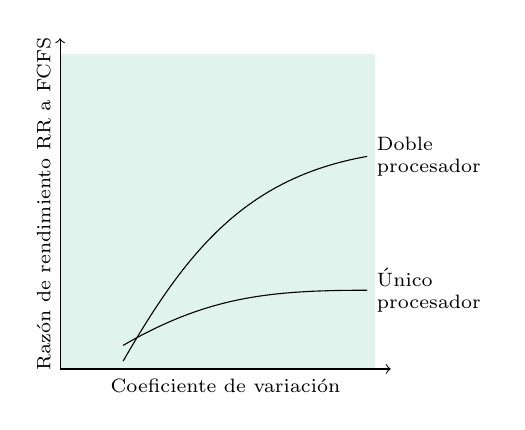
\begin{tikzpicture}[font=\scriptsize]
      \fill[white!95!blue!93!green] (0,0) rectangle (4,4);
      \draw[->] (0,0) -- node[below]{Coeficiente de variación} (4.2,0);
      \draw[->] (0,0) -- node[above,sloped]{Razón de rendimiento RR a FCFS} (0,4.2);
      \draw (0.8,0.3) to[out=30,in=180] (3.9,1) node[right,text width=1.4cm]{Único\\procesador};
      \draw (0.8,0.1) to[out=60,in=190] (3.9,2.7) node[right,text width=1.4cm]{Doble\\procesador};
    \end{tikzpicture}
    \caption{Comparación de RR y FCFS.}
  \end{subfigure}
  \hspace{5mm}
  \begin{subfigure}[c]{0.45\textwidth}
    \centering
    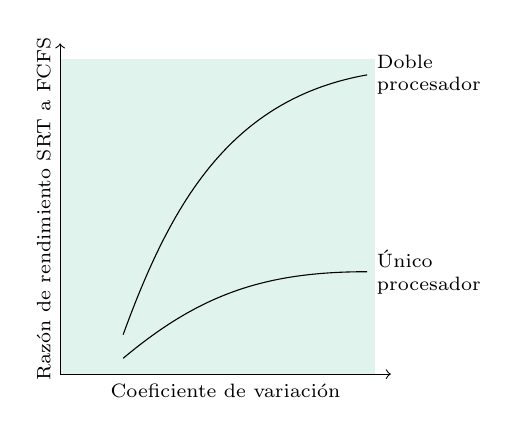
\begin{tikzpicture}[font=\scriptsize]
      \fill[white!95!blue!93!green] (0,0) rectangle (4,4);
      \draw[->] (0,0) -- node[below]{Coeficiente de variación} (4.2,0);
      \draw[->] (0,0) -- node[above,sloped]{Razón de rendimiento SRT a FCFS} (0,4.2);
      \draw (0.8,0.2) to[out=40,in=180] (3.9,1.3) node[right,text width=1.4cm]{Único\\procesador};
      \draw (0.8,0.5) to[out=70,in=190] (3.9,3.8) node[right,text width=1.4cm]{Doble\\procesador};
    \end{tikzpicture}
    \caption{Comparación de SRT y FCFS.}
  \end{subfigure}
  \caption{Comparación del rendimiento de distintos algoritmos de planificación en sistemas con uno y varios procesadores. A medida que aumenta el número de procesadores, las diferencias entre algoritmos como FCFS y Round Robin disminuyen, haciendo que políticas simples sean suficientes en muchos casos.}
\end{figure}

\subsection{Planificación de hilos}

Los hilos permiten separar la ejecución del resto de los recursos de un proceso, posibilitando que varias tareas de una misma aplicación se ejecuten concurrentemente dentro del mismo espacio de direcciones.

En un sistema uniprocesador, los hilos mejoran la estructura de los programas y permiten solapar operaciones de E/S con cómputo, con un costo de cambio de contexto inferior al de los procesos. En un multiprocesador, además, permiten explotar el paralelismo real ejecutando simultáneamente distintos hilos de una misma aplicación. En aplicaciones con alta interacción entre hilos (granularidad media), la política de planificación influye significativamente en el rendimiento.

Las principales estrategias de planificación de hilos son:
\begin{itemize}
  \item \textit{Compartición de carga (\textit{Load Sharing}):} los hilos se almacenan en una cola global y cualquier procesador libre puede ejecutar el siguiente hilo disponible.
  \item \textit{Planificación por grupos (\textit{Gang Scheduling}):} todos los hilos relacionados de una aplicación se ejecutan simultáneamente en distintos procesadores.
  \item \textit{Asignación dedicada de procesadores:} cada aplicación recibe un conjunto fijo de procesadores durante toda su ejecución, normalmente uno por hilo.
  \item \textit{Planificación dinámica:} el número de hilos asignados a una aplicación puede modificarse durante su ejecución según la carga del sistema.
\end{itemize}

\subsubsection{Compartición de carga}

Es la estrategia más simple y una de las más utilizadas en multiprocesadores. Mantiene una cola global de hilos listos, desde la cual cada procesador obtiene trabajo cuando queda libre.

Sus principales ventajas son:
\begin{itemize}
  \item Distribuye automáticamente la carga entre los procesadores.
  \item No requiere un planificador centralizado.
  \item Puede combinarse con cualquier política de planificación, como FCFS o prioridades.
\end{itemize}
Las políticas más comunes para organizar la cola global son:
\begin{itemize}
  \item \textit{FCFS:} los hilos se ejecutan en orden de llegada hasta bloquearse o finalizar.
  \item \textit{Menor número de hilos primero:} se priorizan las aplicaciones que poseen menos hilos pendientes de ejecución.
  \item \textit{Versión apropiativa:} igual que la anterior, pero un nuevo trabajo puede interrumpir la ejecución de otro con menor prioridad.
\end{itemize}

Estudios experimentales muestran que, en la mayoría de los casos, \textit{FCFS} ofrece un mejor rendimiento que las otras variantes de \textit{Load Sharing}. No obstante, la \textit{Gang Scheduling} suele obtener resultados superiores cuando existe una elevada coordinación entre los hilos.

Las principales desventajas de \textit{Load Sharing} son:
\begin{itemize}
  \item La cola global puede convertirse en un cuello de botella cuando muchos procesadores intentan acceder a ella simultáneamente.
  \item Un hilo apropiado puede reanudarse en un procesador distinto, reduciendo la eficiencia de las memorias caché locales.
  \item Los hilos de una misma aplicación pueden ejecutarse en instantes diferentes, perjudicando el rendimiento cuando requieren sincronización frecuente.
\end{itemize}

Una variante consiste en mantener una cola local para cada procesador y una cola global compartida. Cada procesador consulta primero su cola local, reservada para hilos vinculados a dicho procesador, y luego la cola global. Esta organización mejora la localidad de referencia y facilita la implementación de técnicas como la planificación por grupos.

\subsubsection{Planificación por grupos}

La \textit{planificación por grupos} (Gang Scheduling) consiste en ejecutar simultáneamente, en distintos procesadores, todos los hilos relacionados de una misma aplicación. Esta técnica es especialmente útil en aplicaciones con paralelismo de granularidad media o fina, donde los hilos requieren una sincronización frecuente.

Sus principales ventajas son:
\begin{itemize}
  \item Reduce los bloqueos debidos a la sincronización entre hilos, ya que todos pueden ejecutarse al mismo tiempo.
  \item Disminuye la cantidad de cambios de contexto y, por lo tanto, la sobrecarga de planificación.
  \item Facilita el acceso compartido a recursos, reduciendo el costo de sincronización en determinadas operaciones.
\end{itemize}

Si un hilo necesita sincronizarse con otro que aún no está ejecutándose, deberá esperar hasta que el planificador le asigne un procesador, degradando considerablemente el rendimiento. La planificación por grupos evita este problema al garantizar la ejecución simultánea de todos los hilos cooperantes.

La implementación de esta técnica requiere asignar procesadores a cada aplicación. Una estrategia sencilla consiste en repartir el tiempo de CPU entre las aplicaciones mediante \textit{time slicing}. Sin embargo, asignar el mismo tiempo a todas las aplicaciones puede desperdiciar recursos cuando poseen distinta cantidad de hilos.

Una alternativa más eficiente consiste en asignar tiempo de procesador de forma proporcional al número de hilos de cada aplicación. De este modo se reduce el tiempo en que algunos procesadores permanecen inactivos y se mejora la utilización global del sistema.

\begin{figure}[!ht]
  \centering
  \includegraphics[width=0.7\textwidth]{chapters/03_unit/media/gang_scheduling.pdf}
  \caption{Comparación entre una asignación uniforme del tiempo de CPU y una asignación ponderada por la cantidad de hilos. La planificación ponderada reduce el tiempo en que algunos procesadores permanecen ociosos, mejorando la utilización del multiprocesador.}
\end{figure}

\subsection{Asignación dedicada de procesadores}

La \textit{asignación dedicada de procesadores} es una estrategia extrema de la \textit{Gang Scheduling}. Cuando una aplicación comienza a ejecutarse, se le asigna un conjunto fijo de procesadores, uno por hilo, que permanecen dedicados exclusivamente a dicha aplicación hasta su finalización.

A primera vista esta política parece ineficiente, ya que si un hilo se bloquea por una operación de E/S o por sincronización, el procesador asignado permanece inactivo y no puede ejecutar otros procesos. Sin embargo, presenta dos ventajas importantes:
\begin{itemize}
  \item En sistemas con decenas o cientos de procesadores, maximizar la utilización individual de cada procesador deja de ser el objetivo principal; resulta más importante mejorar el rendimiento global de las aplicaciones.
  \item Al eliminar prácticamente todos los cambios de contexto durante la ejecución de una aplicación, se reduce la sobrecarga del sistema y se mejora significativamente su desempeño.
\end{itemize}
Diversos estudios muestran que el rendimiento disminuye cuando el número de hilos activos supera el número de procesadores disponibles. En ese caso aumenta la frecuencia de apropiaciones (\textit{preemption}) y replanificaciones, lo que provoca:
\begin{itemize}
  \item Mayor cantidad de cambios de contexto.
  \item Esperas por hilos suspendidos dentro de secciones críticas.
  \item Pérdida de eficiencia de la memoria caché.
\end{itemize}

Por ello, una estrategia efectiva consiste en limitar el número de hilos activos al número de procesadores del sistema, especialmente en aplicaciones paralelas que pueden distribuir su trabajo mediante colas de tareas.

La asignación dedicada de procesadores y la \textit{Gang Scheduling} abordan el problema desde la perspectiva de la \textit{asignación de procesadores}. Este problema es análogo a la asignación de marcos de página en memoria: el sistema debe decidir cuántos procesadores asignar a cada aplicación para mantener un rendimiento adecuado.

Se define el \textit{conjunto activo de trabajo} (\textit{activity working set}) como el número mínimo de hilos que deben ejecutarse simultáneamente para que una aplicación progrese eficientemente. Si no se asignan suficientes procesadores pueden aparecer dos problemas:
\begin{itemize}
  \item \textit{Thrashing de procesadores:} los hilos necesarios se suspenden mutuamente de forma reiterada, provocando continuas replanificaciones y bajo rendimiento.
  \item \textit{Fragmentación de procesadores:} quedan procesadores libres, pero en una cantidad insuficiente o con una distribución que impide satisfacer las necesidades de las aplicaciones en espera.
\end{itemize}

Las técnicas de \textit{Gang Scheduling} y asignación dedicada buscan minimizar ambos problemas mediante una asignación más eficiente de los procesadores.

\begin{table}[!ht]
  \centering
  \begin{tabular}{c|c|c}
    \makecell{Número de hilos \\ por aplicación} & 
    \makecell{Multiplicación \\ de matriz} & 
    FFT \\ 
    \hline 
    1 & 1 & 1 \\ 
    2 & 1.8 & 1.8 \\
    4 & 3.8 & 3.8 \\
    8 & 6.5 & 6.1 \\
    12 & 5.2 & 5.1 \\
    16 & 3.9 & 3.8 \\
    20 & 3.3 & 3 \\
    24 & 2.8 & 2.4 \\
  \end{tabular}
  \caption{El rendimiento de aplicaciones paralelas aumenta mientras el número de hilos activos no supere la cantidad de procesadores disponibles. Cuando existen más hilos que procesadores, la sobrecarga por apropiaciones y cambios de contexto degrada significativamente el desempeño.}
\end{table}

\subsubsection{Planificación dinámica}

En la \textit{planificación dinámica}, el número de hilos de una aplicación puede modificarse durante su ejecución. Esto permite que el sistema operativo adapte la asignación de procesadores a la carga del sistema, mejorando la utilización de los recursos.

En este enfoque, tanto el sistema operativo como la aplicación participan en la planificación:
\begin{itemize}
  \item El \textit{sistema operativo} decide cuántos procesadores asignar a cada aplicación.
  \item La \textit{aplicación} decide qué tareas ejecutar con los procesadores asignados y qué hilos suspender cuando pierde procesadores.
\end{itemize}
La asignación de procesadores sigue una política sencilla:
\begin{enumerate}
  \item Si existen procesadores libres, se asignan a la aplicación que los solicita.
  \item Si no hay procesadores disponibles, una nueva aplicación recibe al menos un procesador, retirándolo de otra aplicación que posea más de uno.
  \item Las solicitudes no satisfechas permanecen pendientes hasta que algún procesador quede disponible o la aplicación cancele la solicitud.
  \item Cuando se liberan procesadores, primero se atienden las aplicaciones que aún no poseen ninguno y luego el resto de las solicitudes en orden \textit{FCFS}.
\end{enumerate}

Esta estrategia puede ofrecer un mejor rendimiento que la \textit{Gang Scheduling} o la asignación dedicada de procesadores en aplicaciones capaces de adaptar dinámicamente su paralelismo. Sin embargo, la mayor complejidad y la sobrecarga asociada a este mecanismo pueden reducir parte de sus ventajas.

\subsection{Planificación de hilos en sistemas multinúcleo}

Los sistemas operativos modernos, como Windows y Linux, planifican los hilos en sistemas multinúcleo de forma similar a los multiprocesadores, distribuyendo la carga entre los núcleos para mantenerlos ocupados. Sin embargo, esta estrategia no siempre aprovecha al máximo la arquitectura multinúcleo.

A medida que aumenta el número de núcleos, adquiere mayor importancia reducir los accesos a la memoria principal. Para ello se aprovecha la jerarquía de memorias caché, cuya organización influye directamente en las decisiones de planificación.

En muchas arquitecturas multinúcleo, algunos niveles de caché son privados de cada núcleo mientras que otros son compartidos por grupos de núcleos. En consecuencia, la ubicación de los hilos puede afectar significativamente el rendimiento.

\begin{figure}[!ht]
    \centering
    \includegraphics[width=0.8\textwidth]{chapters/03_unit/media/cache_levels.pdf}
    \caption{Ejemplo de jerarquía de caché en un procesador multinúcleo. Cada núcleo posee una caché L1 privada, algunos grupos de núcleos comparten una caché L2 y todos los núcleos comparten una caché L3. La planificación de hilos debe considerar esta organización para mejorar la localidad y reducir la contención de caché.}
\end{figure}

Se distinguen dos situaciones principales:
\begin{itemize}
  \item \textit{Compartición cooperativa de recursos:} varios hilos acceden a los mismos datos. Conviene ejecutarlos en núcleos que compartan caché para aprovechar la localidad de referencia y reducir los accesos a memoria principal.
  \item \textit{Contención de recursos:} varios hilos compiten por el espacio de una misma caché compartida. En este caso es preferible distribuirlos entre núcleos que no compartan caché para evitar reemplazos frecuentes y degradación del rendimiento.
\end{itemize}
Por ello, la planificación en sistemas multinúcleo debe equilibrar dos objetivos: mantener los núcleos ocupados y optimizar el uso de la memoria caché. El desarrollo de algoritmos de planificación sensibles a la jerarquía de caché (\textit{cache-aware scheduling}) y a la contención (\textit{contention-aware scheduling}) constituye un área activa de investigación.


